\section{A nossa visão}\label{sec:vision}

A metáfora que melhor ilustra o nosso sistema é "um quadro de cortiça que se atualiza sozinho, com ajuda de IA".
Neste sistema, o quadro de cortiça é um conjunto de links que o jovem juntar na aplicação e, ao ir analisando os links frequentemente, a IA lê-os e reporta alterações de preço, taxas escondidas ou pressão para comprar enganosa.
Para um utilizador que pague uma versão premium, tal como o agente, este sistema permite ter vários quadros de cortiça ao mesmo tempo (um para cada cliente que ele tenha) e uma melhor IA para fazer esta atualização.
Além disso, também permite guardar opções de fornecedores exclusivos, que não estão disponíveis online.

A seguinte imagem mostra uma visão do nosso sistema:

\begin{figure}[!h]
    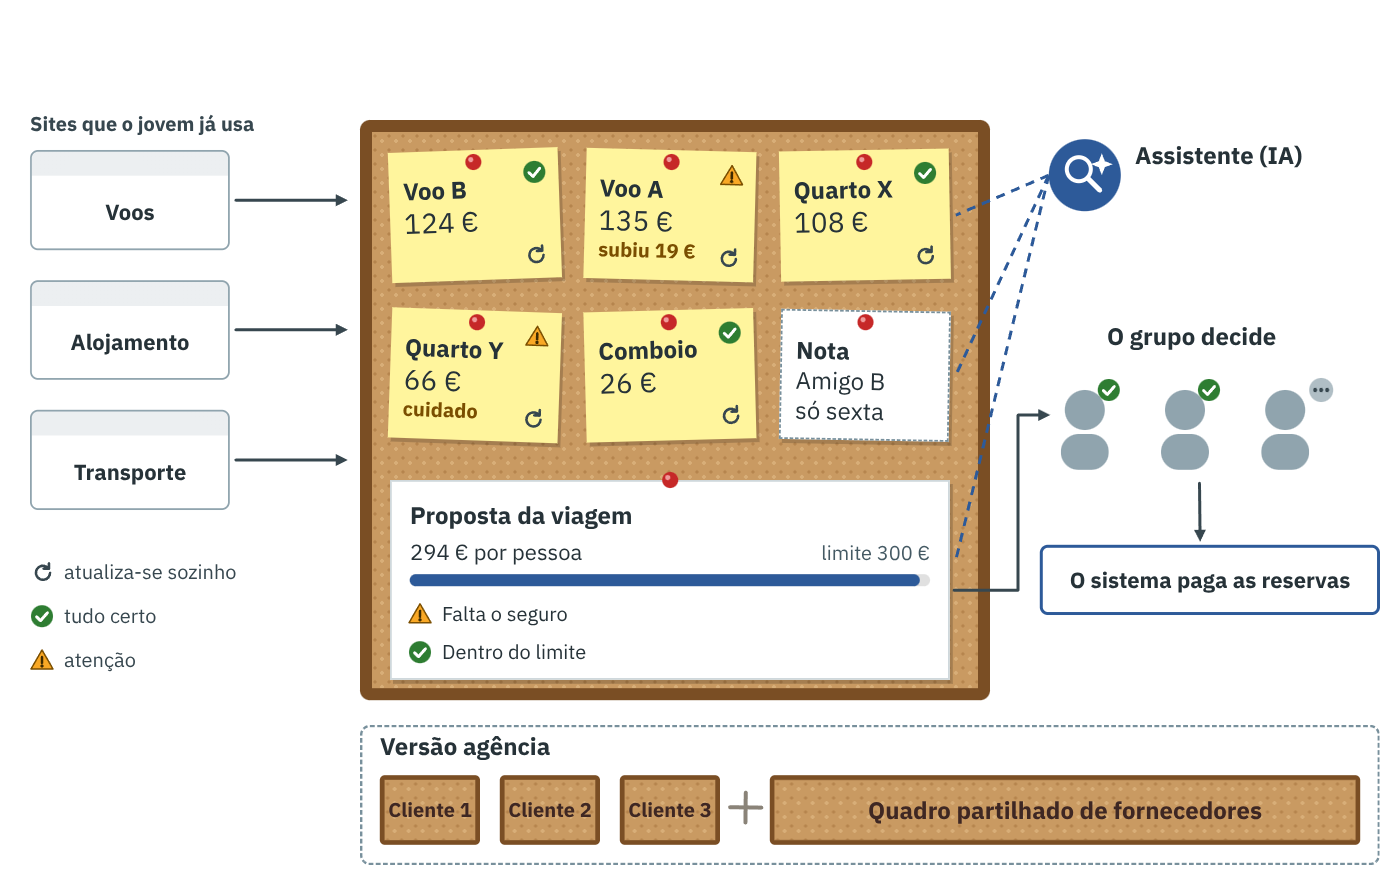
\includegraphics[width=\linewidth]{figuras/vision.png}
    \caption{Roamly: um quadro de cortiça que se atualiza sozinho}
\end{figure}